\section{Mikołaj Kraczek}
\label{sec:Mikołaj}

\subsection{Wyrazenie matematyczne}
    Kazdy chyba teskni za czasami kiedy uczylismy sie smiesznych z perspektywy czasu iloczynow skroconego mnozenia: \[(x+y)^2=x^2+2xy+y^2\]
\subsection{Zdjecie}
    Stare radzieckie bajki mialy swoj swoisty klimat \ref{fig:gigachad}
    \begin{figure}[h]
        \centering
        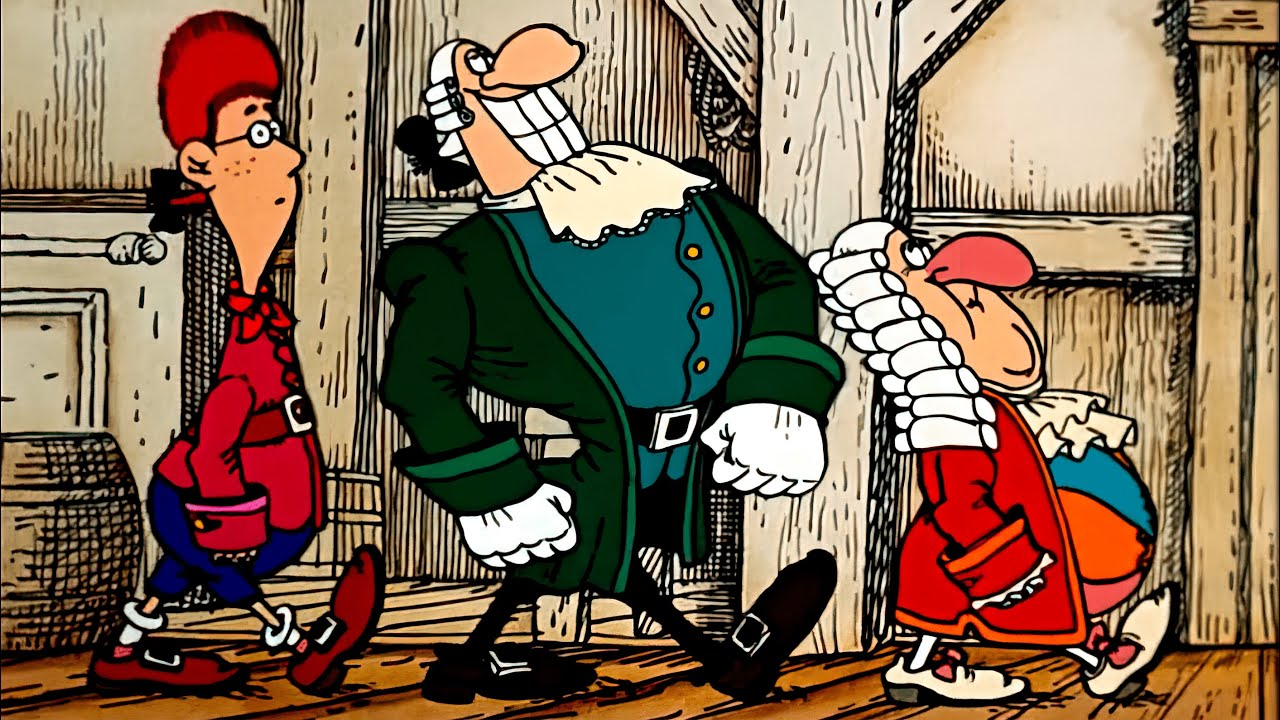
\includegraphics[width=1\textwidth]{pictures/gigachad.jpg}
        \caption{Najlepsza bajka ever}
        \label{fig:gigachad}
    \end{figure}
    \newpage
\subsection{Tabela}
    Przykladowa wygenerowana tabela
    \input{tables/tabela_MikołajKraczek}
\subsection{Listy}
    \subsubsection{Lista numerowana}
        \begin{enumerate}
            \item el. Nr.1
            \item el. Nr.2
            \begin{enumerate}
                \item z.e
            \end{enumerate}
        \end{enumerate}
    \subsubsection{Lista nienumerowana}
        \begin{itemize}
            \item el. Nr.1
            \item el. Nr.2
            \begin{itemize}
                \item e.z
            \end{itemize}
        \end{itemize}
\subsection{Krotki tekst}
\textbf{pogrubiony} \textit{pochylony} \\
    \underline{ podkreslony}
